\documentclass{standalone}
\usepackage{tikz}
\usetikzlibrary{patterns, positioning}
\usepackage[sfdefault]{ClearSans} %% option 'sfdefault' activates Clear Sans as the default text font
\usepackage[T1]{fontenc}

\begin{document}
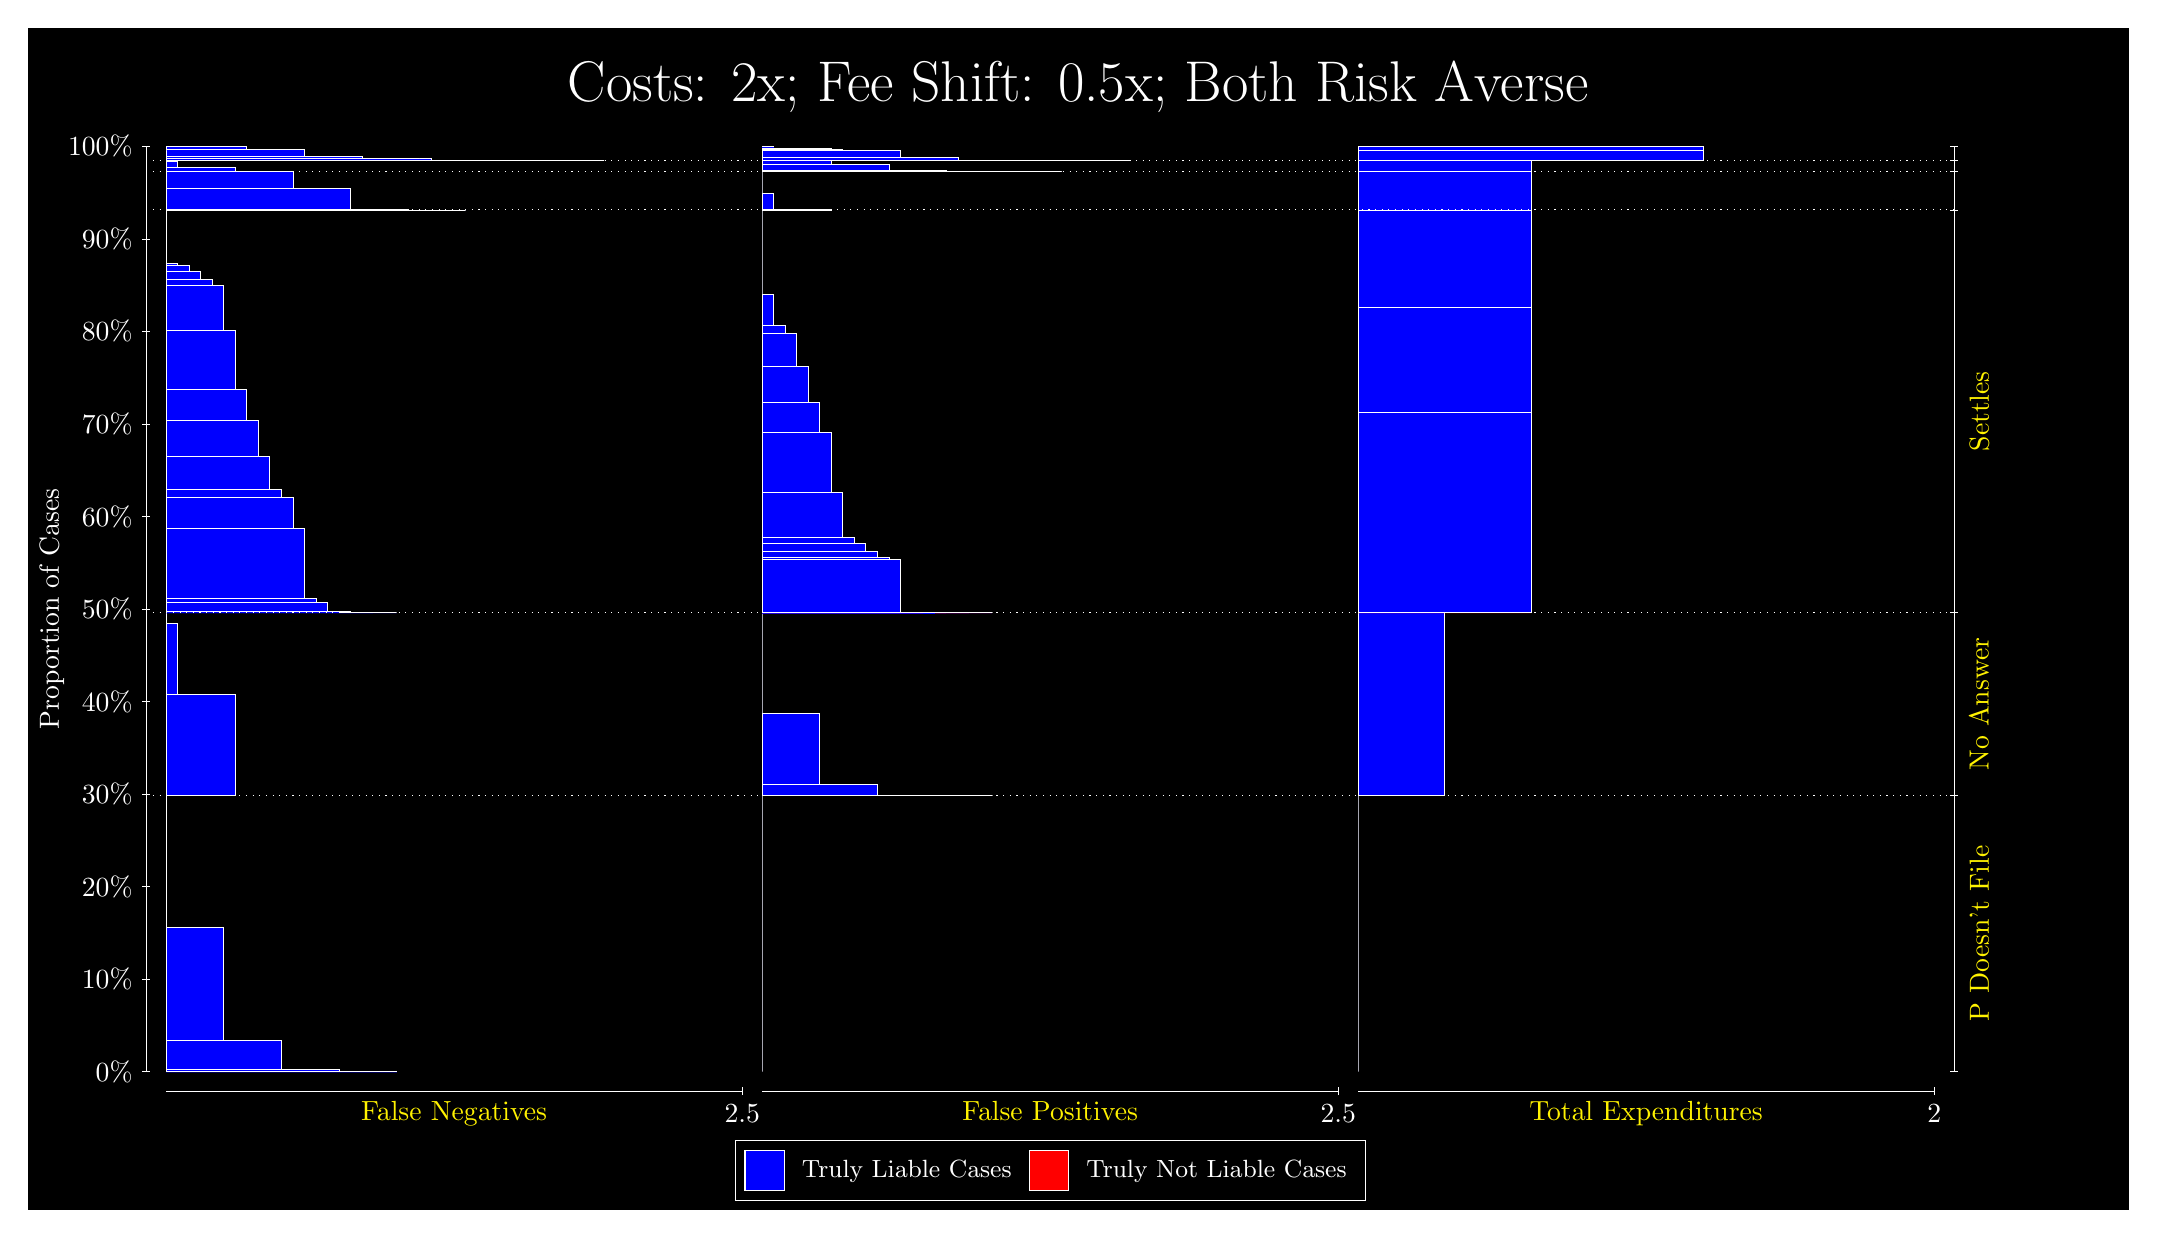
\begin{tikzpicture}
\draw[fill=black] (0,0) rectangle (26.667,15);
\draw[text=white] (0,13.5) rectangle (26.667,15) node[midway] {\huge Costs: 2x; Fee Shift: 0.5x; Both Risk Averse};
\draw[white, very thin] (1.5,1.75) -- (1.5,13.5);
\node[rotate=90, text=white, anchor=center] at (0.3, 7.625) {Proportion of Cases};
\draw[white, very thin] (1.45,1.75) -- (1.55,1.75);
\node[text=white, anchor=east] at (1.45, 1.75) {0\%};
\draw[white, very thin] (1.45,2.925) -- (1.55,2.925);
\node[text=white, anchor=east] at (1.45, 2.925) {10\%};
\draw[white, very thin] (1.45,4.1) -- (1.55,4.1);
\node[text=white, anchor=east] at (1.45, 4.1) {20\%};
\draw[white, very thin] (1.45,5.275) -- (1.55,5.275);
\node[text=white, anchor=east] at (1.45, 5.275) {30\%};
\draw[white, very thin] (1.45,6.45) -- (1.55,6.45);
\node[text=white, anchor=east] at (1.45, 6.45) {40\%};
\draw[white, very thin] (1.45,7.625) -- (1.55,7.625);
\node[text=white, anchor=east] at (1.45, 7.625) {50\%};
\draw[white, very thin] (1.45,8.8) -- (1.55,8.8);
\node[text=white, anchor=east] at (1.45, 8.8) {60\%};
\draw[white, very thin] (1.45,9.975) -- (1.55,9.975);
\node[text=white, anchor=east] at (1.45, 9.975) {70\%};
\draw[white, very thin] (1.45,11.15) -- (1.55,11.15);
\node[text=white, anchor=east] at (1.45, 11.15) {80\%};
\draw[white, very thin] (1.45,12.325) -- (1.55,12.325);
\node[text=white, anchor=east] at (1.45, 12.325) {90\%};
\draw[white, very thin] (1.45,13.5) -- (1.55,13.5);
\node[text=white, anchor=east] at (1.45, 13.5) {100\%};

\draw[white, very thin] (24.457,1.75) -- (24.457,13.5);
\draw[white, very thin] (24.407,1.75) -- (24.507,1.75);
\node[anchor=west] at (24.407, 1.75) {};
\draw[white, very thin] (24.407,5.256) -- (24.507,5.256);
\node[anchor=west] at (24.407, 5.256) {};
\draw[white, very thin] (24.407,7.5779) -- (24.507,7.5779);
\node[anchor=west] at (24.407, 7.5779) {};
\draw[white, very thin] (24.407,12.693) -- (24.507,12.693);
\node[anchor=west] at (24.407, 12.693) {};
\draw[white, very thin] (24.407,13.183) -- (24.507,13.183);
\node[anchor=west] at (24.407, 13.183) {};
\draw[white, very thin] (24.407,13.321) -- (24.507,13.321);
\node[anchor=west] at (24.407, 13.321) {};
\draw[white, very thin] (24.407,13.5) -- (24.507,13.5);
\node[anchor=west] at (24.407, 13.5) {};

\draw[white, very thin, fill=blue] (1.75,1.75) rectangle (4.6775,1.7502);
\draw[white, very thin, fill=blue] (1.75,1.7502) rectangle (3.9457,1.7761);
\draw[white, very thin, fill=blue] (1.75,1.7761) rectangle (3.2138,2.1444);
\draw[white, very thin, fill=blue] (1.75,2.1444) rectangle (2.4819,3.5799);
\draw[white, very thin, fill=red] (1.75,3.5799) rectangle (1.75,3.5799);
\draw[white, very thin, fill=blue] (1.75,3.5799) rectangle (1.75,5.256);
\draw[white, very thin, fill=blue] (1.75,5.256) rectangle (2.6283,6.5357);
\draw[white, very thin, fill=blue] (1.75,6.5357) rectangle (1.8964,7.4413);
\draw[white, very thin, fill=red] (1.75,7.4413) rectangle (1.75,7.4413);
\draw[white, very thin, fill=blue] (1.75,7.4413) rectangle (1.75,7.5779);
\draw[white, very thin, fill=blue] (1.75,7.5779) rectangle (4.6775,7.5779);
\draw[white, very thin, fill=blue] (1.75,7.5779) rectangle (4.3848,7.578);
\draw[white, very thin, fill=blue] (1.75,7.578) rectangle (4.092,7.5893);
\draw[white, very thin, fill=blue] (1.75,7.5893) rectangle (3.9457,7.5898);
\draw[white, very thin, fill=blue] (1.75,7.5898) rectangle (3.7993,7.7089);
\draw[white, very thin, fill=blue] (1.75,7.7089) rectangle (3.6529,7.7627);
\draw[white, very thin, fill=blue] (1.75,7.7627) rectangle (3.5065,8.6486);
\draw[white, very thin, fill=blue] (1.75,8.6486) rectangle (3.3602,9.0445);
\draw[white, very thin, fill=blue] (1.75,9.0445) rectangle (3.2138,9.142);
\draw[white, very thin, fill=blue] (1.75,9.142) rectangle (3.0674,9.5589);
\draw[white, very thin, fill=blue] (1.75,9.5589) rectangle (2.921,10.017);
\draw[white, very thin, fill=blue] (1.75,10.017) rectangle (2.7746,10.409);
\draw[white, very thin, fill=blue] (1.75,10.409) rectangle (2.6283,11.166);
\draw[white, very thin, fill=blue] (1.75,11.166) rectangle (2.4819,11.73);
\draw[white, very thin, fill=blue] (1.75,11.73) rectangle (2.3355,11.809);
\draw[white, very thin, fill=blue] (1.75,11.809) rectangle (2.1891,11.916);
\draw[white, very thin, fill=blue] (1.75,11.916) rectangle (2.0428,11.991);
\draw[white, very thin, fill=blue] (1.75,11.991) rectangle (1.8964,12.019);
\draw[white, very thin, fill=red] (1.75,12.019) rectangle (1.75,12.019);
\draw[white, very thin, fill=blue] (1.75,12.019) rectangle (1.75,12.693);
\draw[white, very thin, fill=blue] (1.75,12.693) rectangle (5.5558,12.693);
\draw[white, very thin, fill=blue] (1.75,12.693) rectangle (4.8239,12.699);
\draw[white, very thin, fill=blue] (1.75,12.699) rectangle (4.092,12.973);
\draw[white, very thin, fill=blue] (1.75,12.973) rectangle (3.3602,13.18);
\draw[white, very thin, fill=blue] (1.75,13.18) rectangle (2.6283,13.183);
\draw[white, very thin, fill=red] (1.75,13.183) rectangle (1.75,13.183);
\draw[white, very thin, fill=blue] (1.75,13.183) rectangle (2.6283,13.235);
\draw[white, very thin, fill=blue] (1.75,13.235) rectangle (1.8964,13.314);
\draw[white, very thin, fill=red] (1.75,13.314) rectangle (1.75,13.314);
\draw[white, very thin, fill=blue] (1.75,13.314) rectangle (1.75,13.321);
\draw[white, very thin, fill=blue] (1.75,13.321) rectangle (7.3123,13.321);
\draw[white, very thin, fill=blue] (1.75,13.321) rectangle (6.5805,13.321);
\draw[white, very thin, fill=blue] (1.75,13.321) rectangle (5.8486,13.325);
\draw[white, very thin, fill=blue] (1.75,13.325) rectangle (5.7022,13.325);
\draw[white, very thin, fill=blue] (1.75,13.325) rectangle (5.1167,13.348);
\draw[white, very thin, fill=blue] (1.75,13.348) rectangle (4.9703,13.348);
\draw[white, very thin, fill=blue] (1.75,13.348) rectangle (4.3848,13.354);
\draw[white, very thin, fill=blue] (1.75,13.354) rectangle (4.2384,13.373);
\draw[white, very thin, fill=blue] (1.75,13.373) rectangle (3.6529,13.373);
\draw[white, very thin, fill=blue] (1.75,13.373) rectangle (3.5065,13.457);
\draw[white, very thin, fill=blue] (1.75,13.457) rectangle (2.921,13.457);
\draw[white, very thin, fill=blue] (1.75,13.457) rectangle (2.7746,13.498);
\draw[white, very thin, fill=blue] (1.75,13.498) rectangle (2.0428,13.5);
\draw[white, very thin, fill=red] (1.75,13.5) rectangle (1.75,13.5);
\draw[white, very thin, fill=blue] (1.75,13.5) rectangle (1.75,13.5);
\draw[white, very thin, fill=red] (9.3189,1.75) rectangle (9.3189,1.75);
\draw[white, very thin, fill=blue] (9.3189,1.75) rectangle (9.3189,5.256);
\draw[white, very thin, fill=red] (9.3189,5.256) rectangle (12.246,5.256);
\draw[white, very thin, fill=blue] (9.3189,5.256) rectangle (12.246,5.256);
\draw[white, very thin, fill=blue] (9.3189,5.256) rectangle (11.515,5.2562);
\draw[white, very thin, fill=blue] (9.3189,5.2562) rectangle (10.783,5.3927);
\draw[white, very thin, fill=blue] (9.3189,5.3927) rectangle (10.051,6.2982);
\draw[white, very thin, fill=blue] (9.3189,6.2982) rectangle (9.3189,7.5779);
\draw[white, very thin, fill=red] (9.3189,7.5779) rectangle (12.246,7.5779);
\draw[white, very thin, fill=blue] (9.3189,7.5779) rectangle (12.246,7.5779);
\draw[white, very thin, fill=red] (9.3189,7.5779) rectangle (11.954,7.5779);
\draw[white, very thin, fill=blue] (9.3189,7.5779) rectangle (11.954,7.5779);
\draw[white, very thin, fill=red] (9.3189,7.5779) rectangle (11.661,7.5779);
\draw[white, very thin, fill=blue] (9.3189,7.5779) rectangle (11.661,7.578);
\draw[white, very thin, fill=blue] (9.3189,7.578) rectangle (11.515,7.5796);
\draw[white, very thin, fill=red] (9.3189,7.5796) rectangle (11.368,7.5796);
\draw[white, very thin, fill=blue] (9.3189,7.5796) rectangle (11.368,7.5807);
\draw[white, very thin, fill=blue] (9.3189,7.5807) rectangle (11.222,7.5819);
\draw[white, very thin, fill=red] (9.3189,7.5819) rectangle (11.075,7.5819);
\draw[white, very thin, fill=blue] (9.3189,7.5819) rectangle (11.075,8.2522);
\draw[white, very thin, fill=blue] (9.3189,8.2522) rectangle (10.929,8.2806);
\draw[white, very thin, fill=blue] (9.3189,8.2806) rectangle (10.783,8.3552);
\draw[white, very thin, fill=blue] (9.3189,8.3552) rectangle (10.636,8.4628);
\draw[white, very thin, fill=blue] (9.3189,8.4628) rectangle (10.49,8.541);
\draw[white, very thin, fill=blue] (9.3189,8.541) rectangle (10.344,9.1058);
\draw[white, very thin, fill=blue] (9.3189,9.1058) rectangle (10.197,9.8627);
\draw[white, very thin, fill=blue] (9.3189,9.8627) rectangle (10.051,10.255);
\draw[white, very thin, fill=blue] (9.3189,10.255) rectangle (9.9044,10.712);
\draw[white, very thin, fill=blue] (9.3189,10.712) rectangle (9.758,11.129);
\draw[white, very thin, fill=blue] (9.3189,11.129) rectangle (9.6116,11.227);
\draw[white, very thin, fill=blue] (9.3189,11.227) rectangle (9.4652,11.623);
\draw[white, very thin, fill=blue] (9.3189,11.623) rectangle (9.3189,12.693);
\draw[white, very thin, fill=red] (9.3189,12.693) rectangle (10.197,12.693);
\draw[white, very thin, fill=blue] (9.3189,12.693) rectangle (10.197,12.696);
\draw[white, very thin, fill=blue] (9.3189,12.696) rectangle (9.4652,12.904);
\draw[white, very thin, fill=blue] (9.3189,12.904) rectangle (9.3189,13.183);
\draw[white, very thin, fill=red] (9.3189,13.183) rectangle (13.125,13.183);
\draw[white, very thin, fill=blue] (9.3189,13.183) rectangle (13.125,13.183);
\draw[white, very thin, fill=blue] (9.3189,13.183) rectangle (12.393,13.183);
\draw[white, very thin, fill=blue] (9.3189,13.183) rectangle (11.661,13.19);
\draw[white, very thin, fill=blue] (9.3189,13.19) rectangle (10.929,13.269);
\draw[white, very thin, fill=blue] (9.3189,13.269) rectangle (10.197,13.321);
\draw[white, very thin, fill=red] (9.3189,13.321) rectangle (14.003,13.321);
\draw[white, very thin, fill=blue] (9.3189,13.321) rectangle (14.003,13.321);
\draw[white, very thin, fill=red] (9.3189,13.321) rectangle (13.271,13.321);
\draw[white, very thin, fill=blue] (9.3189,13.321) rectangle (13.271,13.321);
\draw[white, very thin, fill=red] (9.3189,13.321) rectangle (12.539,13.321);
\draw[white, very thin, fill=blue] (9.3189,13.321) rectangle (12.539,13.323);
\draw[white, very thin, fill=blue] (9.3189,13.323) rectangle (11.807,13.365);
\draw[white, very thin, fill=red] (9.3189,13.365) rectangle (11.807,13.365);
\draw[white, very thin, fill=blue] (9.3189,13.365) rectangle (11.807,13.365);
\draw[white, very thin, fill=red] (9.3189,13.365) rectangle (11.661,13.365);
\draw[white, very thin, fill=blue] (9.3189,13.365) rectangle (11.661,13.365);
\draw[white, very thin, fill=blue] (9.3189,13.365) rectangle (11.075,13.447);
\draw[white, very thin, fill=blue] (9.3189,13.447) rectangle (11.075,13.448);
\draw[white, very thin, fill=red] (9.3189,13.448) rectangle (10.929,13.448);
\draw[white, very thin, fill=blue] (9.3189,13.448) rectangle (10.929,13.448);
\draw[white, very thin, fill=blue] (9.3189,13.448) rectangle (10.344,13.457);
\draw[white, very thin, fill=blue] (9.3189,13.457) rectangle (10.344,13.467);
\draw[white, very thin, fill=blue] (9.3189,13.467) rectangle (10.197,13.473);
\draw[white, very thin, fill=red] (9.3189,13.473) rectangle (10.197,13.473);
\draw[white, very thin, fill=blue] (9.3189,13.473) rectangle (10.197,13.473);
\draw[white, very thin, fill=blue] (9.3189,13.473) rectangle (9.6116,13.473);
\draw[white, very thin, fill=blue] (9.3189,13.473) rectangle (9.6116,13.473);
\draw[white, very thin, fill=blue] (9.3189,13.473) rectangle (9.4652,13.495);
\draw[white, very thin, fill=blue] (9.3189,13.495) rectangle (9.4652,13.496);
\draw[white, very thin, fill=blue] (9.3189,13.496) rectangle (9.3189,13.5);
\draw[white, very thin, fill=red] (16.888,1.75) rectangle (16.888,1.75);
\draw[white, very thin, fill=blue] (16.888,1.75) rectangle (16.888,5.256);
\draw[white, very thin, fill=red] (16.888,5.256) rectangle (17.986,5.256);
\draw[white, very thin, fill=blue] (16.888,5.256) rectangle (17.986,7.5779);
\draw[white, very thin, fill=red] (16.888,7.5779) rectangle (19.083,7.5779);
\draw[white, very thin, fill=blue] (16.888,7.5779) rectangle (19.083,10.125);
\draw[white, very thin, fill=red] (16.888,10.125) rectangle (19.083,10.125);
\draw[white, very thin, fill=blue] (16.888,10.125) rectangle (19.083,11.458);
\draw[white, very thin, fill=red] (16.888,11.458) rectangle (19.083,11.458);
\draw[white, very thin, fill=blue] (16.888,11.458) rectangle (19.083,12.693);
\draw[white, very thin, fill=red] (16.888,12.693) rectangle (19.083,12.693);
\draw[white, very thin, fill=blue] (16.888,12.693) rectangle (19.083,13.183);
\draw[white, very thin, fill=red] (16.888,13.183) rectangle (19.083,13.183);
\draw[white, very thin, fill=blue] (16.888,13.183) rectangle (19.083,13.321);
\draw[white, very thin, fill=red] (16.888,13.321) rectangle (21.279,13.321);
\draw[white, very thin, fill=blue] (16.888,13.321) rectangle (21.279,13.456);
\draw[white, very thin, fill=red] (16.888,13.456) rectangle (21.279,13.456);
\draw[white, very thin, fill=blue] (16.888,13.456) rectangle (21.279,13.5);
\draw[white, dotted] (1.5,5.256) -- (24.457,5.256);
\draw[white, dotted] (1.5,7.5779) -- (24.457,7.5779);
\draw[white, dotted] (1.5,12.693) -- (24.457,12.693);
\draw[white, dotted] (1.5,13.183) -- (24.457,13.183);
\draw[white, dotted] (1.5,13.321) -- (24.457,13.321);
\draw[white, very thin] (1.75,1.5) -- (9.0689,1.5);
\node[text=yellow, anchor=north] at (5.4094, 1.5) {False Negatives};
\draw[white, very thin] (9.0689,1.45) -- (9.0689,1.55);
\node[text=white, anchor=north] at (9.0689, 1.45) {2.5};

\draw[white, very thin] (9.3189,1.5) -- (16.638,1.5);
\node[text=yellow, anchor=north] at (12.978, 1.5) {False Positives};
\draw[white, very thin] (16.638,1.45) -- (16.638,1.55);
\node[text=white, anchor=north] at (16.638, 1.45) {2.5};

\draw[white, very thin] (16.888,1.5) -- (24.207,1.5);
\node[text=yellow, anchor=north] at (20.547, 1.5) {Total Expenditures};
\draw[white, very thin] (24.207,1.45) -- (24.207,1.55);
\node[text=white, anchor=north] at (24.207, 1.45) {2};

\node[text=yellow, centered, rotate=90] at (24.777, 3.503) {P Doesn't File};
\node[text=yellow, centered, rotate=90] at (24.777, 6.417) {No Answer};
\node[text=yellow, centered, rotate=90] at (24.777, 10.136) {Settles};




\draw (12.978300999999998,1.5) node[draw=none] (baseCoordinate) {};
\begin{scope}[align=center]
        \matrix[scale=0.5, draw=white, below=0.5cm of baseCoordinate, nodes={draw}, column sep=0.1cm]{
            \node[rectangle, draw, minimum width=0.5cm, minimum height=0.5cm, fill=blue] {}; &
            \node[draw=none, font=\small, text=white] (B) {Truly Liable Cases}; &
            \node[rectangle, draw, minimum width=0.5cm, minimum height=0.5cm, fill=red] {}; &
            \node[draw=none, font=\small, text=white] (B) {Truly Not Liable Cases}; \\
            };
\end{scope}

\end{tikzpicture}
\end{document}